\chapter{Modelli e Funzionamento}\label{cap:modefunz}
\section{Blazor Server}\label{sez:bserver}
Il primo dei modelli ufficialmente rilasciati e per il quale si pu\`o gi\`a ricevere supporto in produzione, sin da settembre 2019\cite{blazorServerRelease}, \`e Blazor Server.

Un'applicazione Blazor Server ospita i componenti Blazor lato Server e gestisce le interazioni dell'utente con la UI attraverso una connessione in tempo reale sfruttando SignalR, come visibile nella figura \ref{fig:BlazorServer}.

Per "componente" si intende un pezzo di UI autonomo, come una pagina, una finestra modale o un form da compilare.
Un componente include quindi sia HTML che la logica necessaria per iniettarci dei dati o per rispondere ad eventi della UI. 
I componenti sono flessibili e leggeri. Possono essere annidati, riutilizzati, e condivisi tra progetti\cite{whatIsAComponent}.

SignalR invece \`e una libreria di software open-source sviluppata da Microsoft, che facilita l'interazione tra Client e Server, specialmente quando si necessita di mandare messaggi dal server ad uno o pi\`u client con un'alta frequenza~\cite{signalR}.
SignalR mette a disposizione delle API che permettono al codice del server di eseguire Remote Procedure Calls(RPC), in particolare \`e utilizzato per inviare messaggi real-time ad uno o pi\`u client connessi all'applicazione contemporaneamente(e.g. in una chat room).
Questa libreria viene sfruttata dal modello Blazor Server per trasmettere al browser di ciascun utente connesso quali modifiche debbano essere applicate al Document Object Model(DOM) perch\`e la UI di ciascun Client rispetti la UI che il server mantiene in memoria.
SignalR supporta le seguenti tre tecniche di gestione per comunicare in tempo reale, in ordine di fallback:
\begin{enumerate}
	\item WebSockets
	\item Server-Sent Events
	\item Long Polling
\end{enumerate}

SignalR sceglie automaticamente il miglior metodo di trasporto disponibile a seconda delle capacit\`a di client e server che stabiliscono la connessione\cite{signalR-ASP.NET}.

\begin{figure}[H]
	\centerline{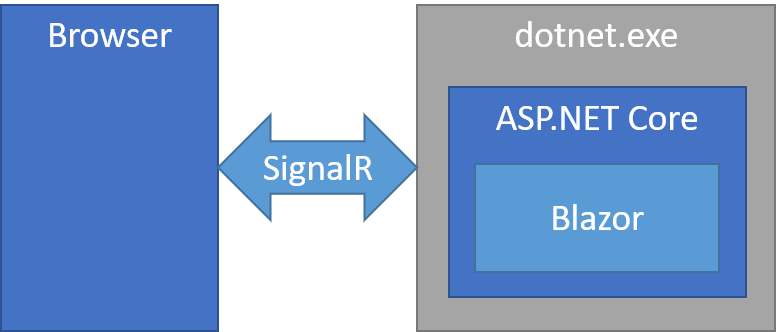
\includegraphics[scale=0.6]{figure/blazor-server.png}}
	\caption{Blazor Server}
	\label{fig:BlazorServer}
\end{figure}

Ci\`o significa che quando un utente scatena un evento, questo viene inviato attraverso la real time connection al server, dove il rispettivo componente di competenza lo gestisce.
Quando l'evento \`e stato gestito, Blazor compara l'output appena generato con quello precedente all'evento, e se presenti manda le sole differenze al browser del client, per poi applicarle al DOM\cite{blazorModelsScenarios}.

Questa caratteristica del modello Blazor Server \`e una fondamentale differenza rispetto a ASP.NET e Razor: le pagine rigenerate ad ogni evento lato server, in precedenza, venivano totalmente rispedite al client, operazione che non richiedeva RAM in modo persistente per ogni utente connesso al server, ma molto meno efficiente in termini di prestazioni.
Blazor Server perci\`o necessita di una connessione stabile e a bassa latenza per funzionare al meglio, e gli scenari offline non sono supportati.
Ci\`o significa anche che la posizione del server sul quale \`e ospitata l'applicazione non pu\`o essere troppo distante dal client che si sta connettendo per garantire un funzionamento senza lag.

Questo modello \`e particolarmente indicato quando si vuole delegare il costo computazionale al server e non ai client che ci si connettono, dato che ci\`o che il client deve computare \`e il solo codice statico scaricato inizialmente, e le differenze di volta in volta ricevute dal server, dove avviene invece la gestione di ogni evento e il calcolo delle differenze tra ci\`o che viene visualizzato prima di un evento e ci\`o che deve cambiare nella User-Interface del client dopo la sua gestione.
Ci\`o rende molto veloce ed efficiente il download iniziale e l'avvio dell'applicazione per gli utenti, il che lo rende il modello pi\`u adatto se le macchine che devono utilizzare l'applicazione sono apparecchi a basso costo, ammesso che siano sempre essere connessi ad internet.

\subsection{BlazorPong - Server}\label{sez:bpongserv}
Un esempio di applicazione scritta utilizzando questo modello \`e BlazorPongServer(BlazorPongServer.sln), appositamente implementata per questo lavoro di tesi e la cui demo e codice sviluppato sono disponibili nel seguente repository su GitHub: \linebreak "https://github.com/MACEL94/BlazorPong".

\begin{figure}[H]
	\centerline{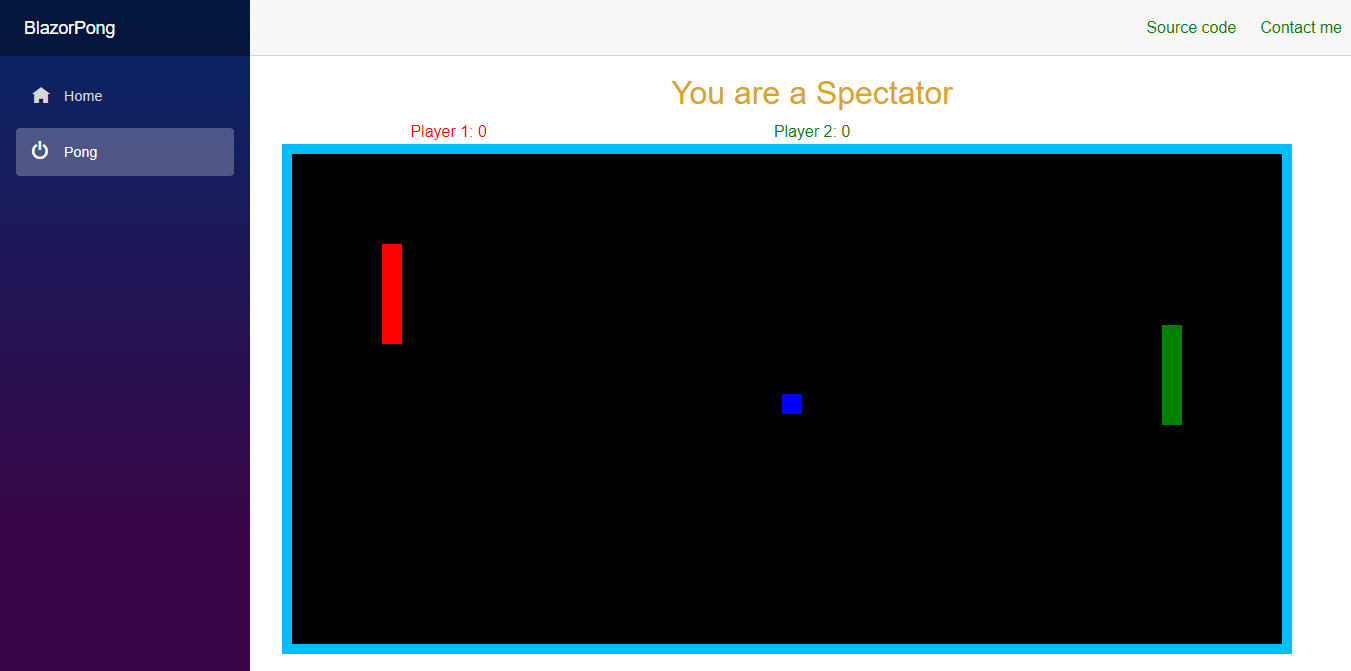
\includegraphics[scale=0.3]{figure/BlazorPong.PNG}}
	\caption{BlazorPong}
	\label{fig:BlazorPong}
\end{figure}

Questa applicazione, visibile nella figura \ref{fig:BlazorPong} permette a due giocatori che si collegano al sito contemporaneamente di giocare, e ai successivi utenti che si collegano di seguire la partita in corso come spettatori in tempo reale.
In questa applicazione \`e stato utilizzato il modello Blazor Server side per vari motivi:
\begin{enumerate}
	\item Il background worker del server che si occupa di aggiornare la posizione della pallina su tutti i client connessi, deve essere eseguito in un unico thread utilizzato per tutti i client.
	\item Il calcolo delle differenze da applicare a ciascun DOM di ciascun utente connesso, per quanto avvenga molto spesso(\`e stato limitato per rendere 60 fps circa), non ha un peso tale da non poter essere eseguito lato server poich\'e l'applicazione \`e molto semplice e di conseguenza leggera.
	Una sola macchina host gratuita come quella che \`e stata utilizzata(su Azure), riesce a far giocare senza problemi due persone con diversi spettatori.
	\`E comunque bene specificare che tutti i test di performance che sono stati fatti sono stati eseguiti in Europa, e che il server utilizzato si trova in Francia.
	\item Essendo la gestione degli eventi server side, il gioco pu\`o essere visualizzato in modalit\`a spettatore senza problemi anche su cellulari non performanti.
\end{enumerate}

Il funzionamento di BlazorPong \`e piuttosto semplice: quando almeno due utenti si collegano all'applicazione e ciascuno ha cliccato play, inizia la partita.
Lato server viene gestito lo spostamento costante della pallina ed eventuali collisioni con muri verticali, orizzontali o con il blocco di uno dei player.
Rispettivamente gli eventi gestiti dal background worker eseguito sul server sono i seguenti:
\begin{enumerate}
	\item Collisione con un muro verticale con conseguente punto per il player che si trova dal lato opposto di quello in cui avviene la collisione;
	\item Collisione con un muro orizzontale con conseguente inversione della velocit\`a di spostamento della pallina sull'asse y;
	\item Collisione con uno dei blocchi dei giocatori con conseguente inversione della velocit\`a di spostamento della pallina sugli assi x ed y;
	\item L'arrivo a 3 punti di uno dei due giocatori o la disconnessione di uno dei due, gestito con l'invio di un messaggio di fine partita contenente il player vincitore a tutti gli utenti connessi.
\end{enumerate}

Ci\`o che invece avviene grazie all'utente, \`e lo spostamento del proprio player attraverso la cattura dell'evento di drag eseguito sul proprio blocco quando lo si trascina.
Ad ogni evento scatenato dall'utente, la connessione SignalR invia l'evento al server, che lo processa e restituisce a tutti gli utenti connessi la nuova posizione.
Viene escluso dall'aggiornamento di posizione del blocco inviato dal server, il solo player che ha scatenato l'evento, poich\'e l'invio delle differenze necessarie per renderizzare la UI aggiornata viene gestito gi\`a da Blazor Server.

\`E importante notare che gi\`a per questa semplice applicazione, il cui sviluppo \`e avvenuto mentre Blazor Server era ancora in preview e che ora è aggiornato all'ultima versione stabile disponibile, Blazor Server ha permesso di utilizzare pochissimo codice Javascript.
Il poco Javascript presente \`e stato necessario per gestire gli eventi client-side che non sono ancora supportati da questo framework, come l'evento "onbeforeunload", che viene scatenato quando il documento che costituisce la pagina sta per essere liberato, evento che necessariamente deve essere intercettato per liberare la sessione del player dal server al momento della chiusura o uscita dal sito.

\pagebreak

\section{Blazor WebAssembly}\label{sez:bwa}
Blazor WebAssembly \`e un modello attualmente in anteprima, e sar\`a ufficialmente rilasciato verso maggio del 2020.

In questo modello il codice della SPA viene scaricato ed eseguito nel browser del client che si collega, come solitamente avviene quando si utilizza un framework moderno per UI come i gi\`a citati Angular, React e Vue.

\begin{figure}[H]
	\centerline{\includegraphics[scale=0.6]{figure/blazor-WebAssembly.png}}
	\caption{Blazor WebAssembly}
	\label{fig:BlazorWebAssembly}
\end{figure}

Vengono quindi scaricati dal client l'applicazione Blazor, le sue dipendenze, ed il runtime .NET necessario per eseguire le DLL.
L'applicazione viene quindi eseguita direttamente nel thread della UI del Browser utilizzato per collegarsi all'applicazione, come visibile nella figura \ref{fig:BlazorWebAssembly}.

L'ambito di esecuzione \`e la stessa sandbox di qualsiasi altra applicazione scritta con javascript, ossia il browser che si sta utilizzando.
Ci\`o \`e molto importante perch\`e significa che potenzialmente un'applicazione web scritta utilizzando Blazor non pu\`o fare niente di pi\`u o di meno di un'applicazione web standard(come ad esempio accedere al file system).
Ogni update alla UI e la relativa gestione, avvengono utilizzando lo stesso processo nel browser.
Per questo modello, blazor.WebAssembly.js \`e il nome dello script Javascript che all'apertura della pagina index si occupa di scaricare il .NET runtime compilato in WebAssembly, l'applicazione e le sue dipendenze, come anche dell'inizializzazione dell'applicazione.

\subsection{CLR e WebAssembly}\label{sez:webAssembly}
In particolare il nome Blazor WebAssembly per questo modello \`e stato scelto perch\`e nel browser di ciascun client che utilizza un'applicazione di questo tipo, viene scaricato ed utilizzato il file "dotnet.wasm"(precedentemente chiamato "mono.wasm").
Questo file contiene il CLR(Common Language Runtime) di Mono, una delle implementazioni del .NET Standard, compilato in WebAssembly e quindi eseguibile dal browser.
Il runtime \`e necessario per poter interpretare ed eseguire i file compilati dell'applicazione(le DLL) e i pacchetti sulla quale si basa, che hanno estensione .dll e come target uno dei framework che implementano il .NET Standard(nel caso di Blazor, .NET Core), come visibile nella figura \ref{fig:CLR}.

\begin{figure}[H]
	\centerline{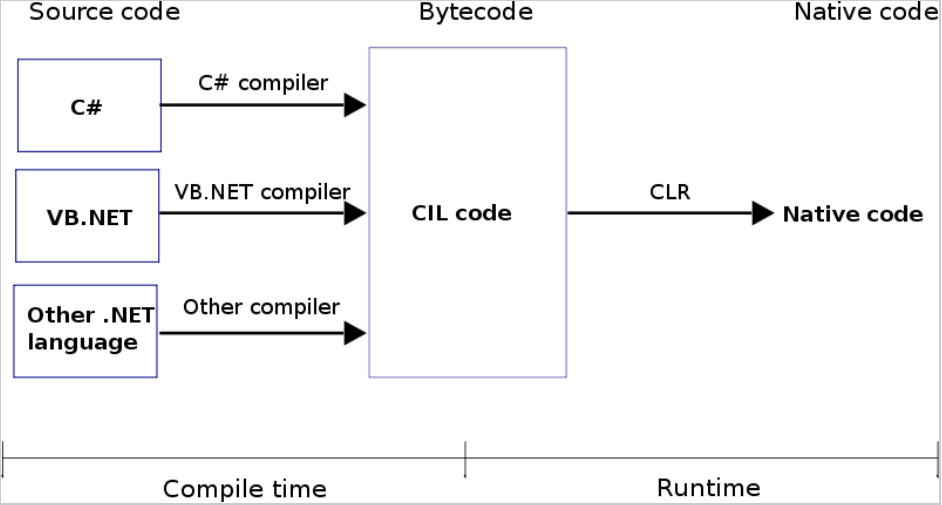
\includegraphics[scale=0.5]{figure/CLR.PNG}}
	\caption{Utilizzo del CLR}
	\label{fig:CLR}
\end{figure}

Il WebAssembly(WASM) \`e un formato per istruzioni binarie creato per essere il target della compilazione di linguaggi ad alto livello come C, C++, Rust\cite{webAssemblyOfficialWebsite}.
L'estensione .wasm \`e quella che \`e stata scelta per i file WASM.
Il progetto per la creazione di WASM \`e nato nel 2015, mentre dal 2017 i browser pi\`u diffusi al mondo come Chrome, Firefox, Edge e Safari si sono impegnati per svilupparlo ed adottarlo\cite{webAssemblySupport}.

\begin{figure}[H]
	\centerline{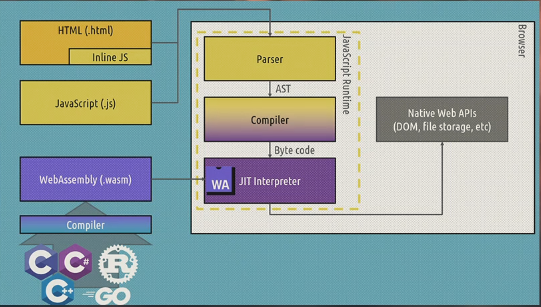
\includegraphics[scale=0.7]{figure/WasmVSJavascript.PNG}}
	\caption{Confronto tra WebAssembly e Javascript}
	\label{fig:WasmVSJavascript}
\end{figure}

Come si pu\`o vedere nella figura \ref{fig:WasmVSJavascript}, uno dei motivi per cui WASM \`e pi\`u veloce di Javascript \`e che non deve essere analizzato e compilato prima di poter essere interpretato, va solamente decompresso e per questo motivo spesso viene definito il byte code per il web.

La compilazione pu\`o avvenire in modalit\`a AOT(Ahead of Time) e non solamente JIT(Just in Time) come per JS, il che si traduce in un sensibile miglioramento delle prestazioni del codice dinamico.
Questa tecnologia \`e ci\`o che rende possibile il funzionamento di Blazor WebAssembly.

\subsection{Blazor PWA}\label{sez:bpwa}
Il passaggio successivo per avvicinarsi a prestazioni e interazioni native per il client, allontanandosi ulteriormente dal modello Blazor Server, \`e chiamato Blazor PWA.
\`E cos\`i chiamato perch\`e in questo modello Blazor, permette di sviluppare l'interfaccia utente di una Progressive Web-App(PWA).

\begin{figure}[H]
	\centerline{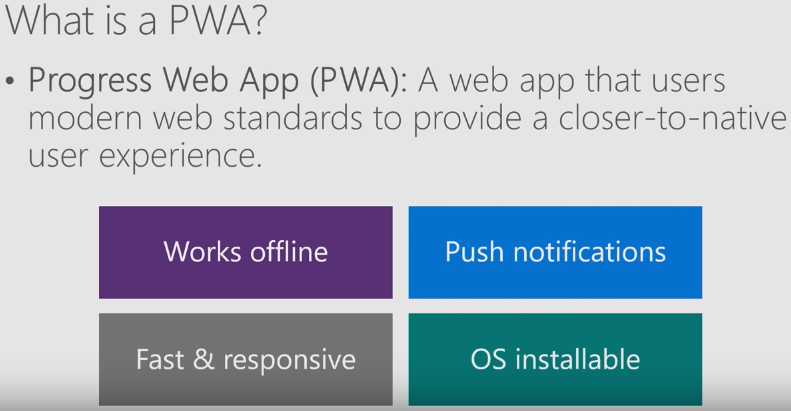
\includegraphics[scale=0.5]{figure/ProgressiveWebApp.png}}
	\caption{Progressive Web Apps}
	\label{fig:WhatIsAPWA}
\end{figure}

Nella figura \ref{fig:WhatIsAPWA} viene riassunto cosa siano le PWA ovvero applicazioni web che hanno la capacit\`a di funzionare anche offline, possono essere scaricate in modo persistente sulla macchina dell'utente che le esegue.
Offrono il vantaggio di una maggiore velocit\`a di esecuzione e la possibilit\`a di sfruttare alcune API native.
Questo modello quindi, pu\`o tornare utile quando la necessit\`a dell'applicazione che si vuole sviluppare \`e quella di utilizzare le notifiche push native del sistema operativo che sta utilizzando il client.

Al momento, per realizzare una PWA utilizzando Blazor, bisogna partire dal modello Blazor WebAssembly aggiungendo un manifesto che descriva le capacit\`a dell'applicazione, i permessi richiesti e l'icona da utilizzare una volta installata, oltre chiaramente a dover implementare l'applicazione in modo che possa lavorare anche offline, basandosi su un service worker\cite{blazorPWA}.

Un'applicazione web infatti per essere considerata una PWA, deve poter essere installata in caso l'utente utilizzi Windows o appuntata nel caso in cui l'utente stia utilizzando un cellulare, e deve supportare l'utilizzo dell'HTTPS, già presente di default nei template forniti per Blazor.

Una cosa molto importante da tenere presente, \`e che le demo esistenti al momento per le PWA scritte in Blazor si basano su browser Chromium Based(Chrome,Edge) e sul sistema operativo Windows per PC e IOS/Android per mobile.
Per ora quindi non tutti i browser supportano queste PWA.

\subsection{BlazorPong - Client e PWA}\label{sez:bpongclient}
Un esempio di applicazione scritta utilizzando il modello Blazor WASM \`e BlazorPongClient(BlazorPongWasm.sln), appositamente implementato per questo lavoro di tesi e la cui demo e codice sviluppato sono disponibili nel seguente repository su GitHub: "https://github.com/MACEL94/BlazorPong".

Questo progetto dimostra come sia possibile condividere il codice dei component e riutilizzarlo, visto che il component visibile al route /pong \`e lo stesso gi\`a presente in BlazorPongServer, spostato in un progetto condiviso e quindi referenziato in entrambi.

Chiaramente l'applicazione in questo caso non \`e costituita da soli file statici, e non pu\`o essere scaricata completamente lato client o servita da un CDN.

Ci\`o che si \`e scelto quindi \`e di spostare la sola logica di render della UI lato Client attraverso il cambio di modello.
La WebApp viene comunque ospitata su un server dove continua ad avvenire la computazione dello spostamento della pallina e il calcolo di eventuali collisioni con muri o player, attraverso l'utilizzo di un background worker come in precedenza.

In questo modello si \`e deciso di integrare anche il service worker che permette di installare l'applicazione in modo da farla sembrare nativa e ricercabile dal men\`u start, ad esempio in Windows.

Ci\`o \`e visibile di seguito nelle immagini \ref{fig:installableBlazorPongWasm}, \ref{fig:searchingBlazorPongWasm} e \ref{fig:installedBlazorPongWasm}.
\begin{figure}[H]
	\centerline{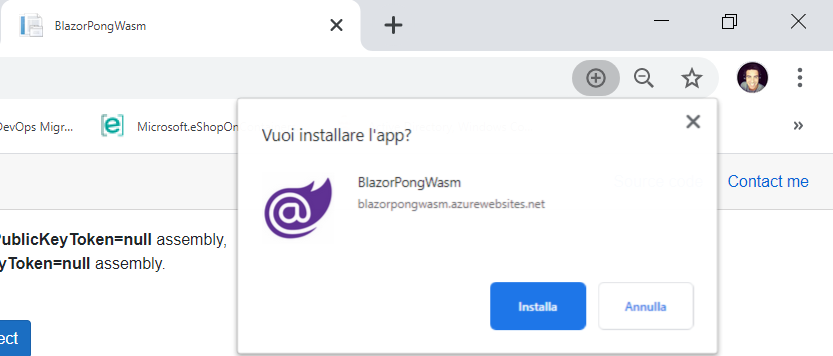
\includegraphics[scale=0.6]{figure/installableBlazorPongWasm.png}}
	\caption{L'utente pu\`o decidere di installare l'applicazione.}
	\label{fig:installableBlazorPongWasm}
\end{figure}

\begin{figure}[H]
	\centerline{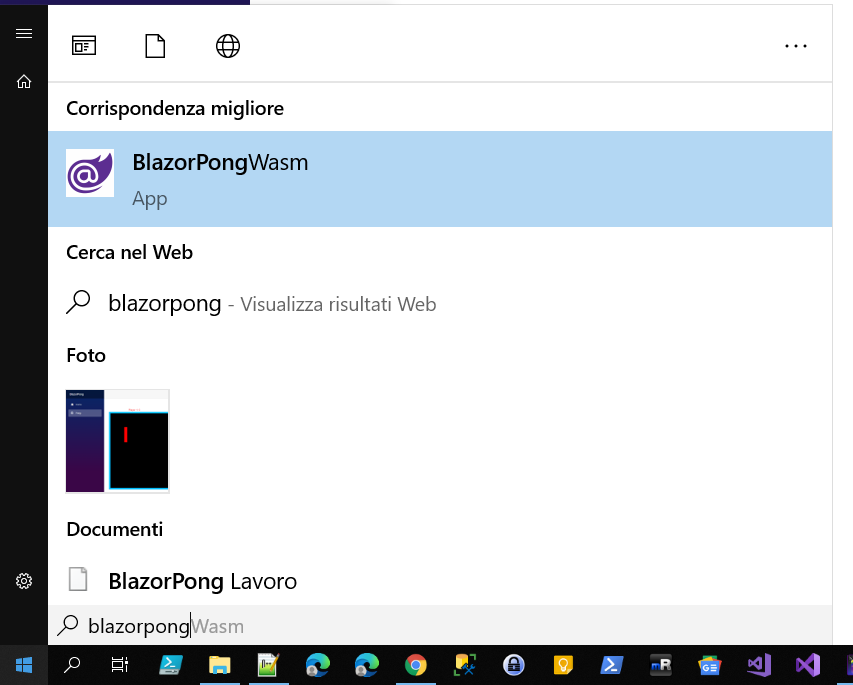
\includegraphics[scale=0.5]{figure/searchingBlazorPongWasm.png}}
	\caption{L'applicazione installata \`e ricercabile dal men\`u start.}
	\label{fig:searchingBlazorPongWasm}
\end{figure}

\begin{figure}[H]
	\centerline{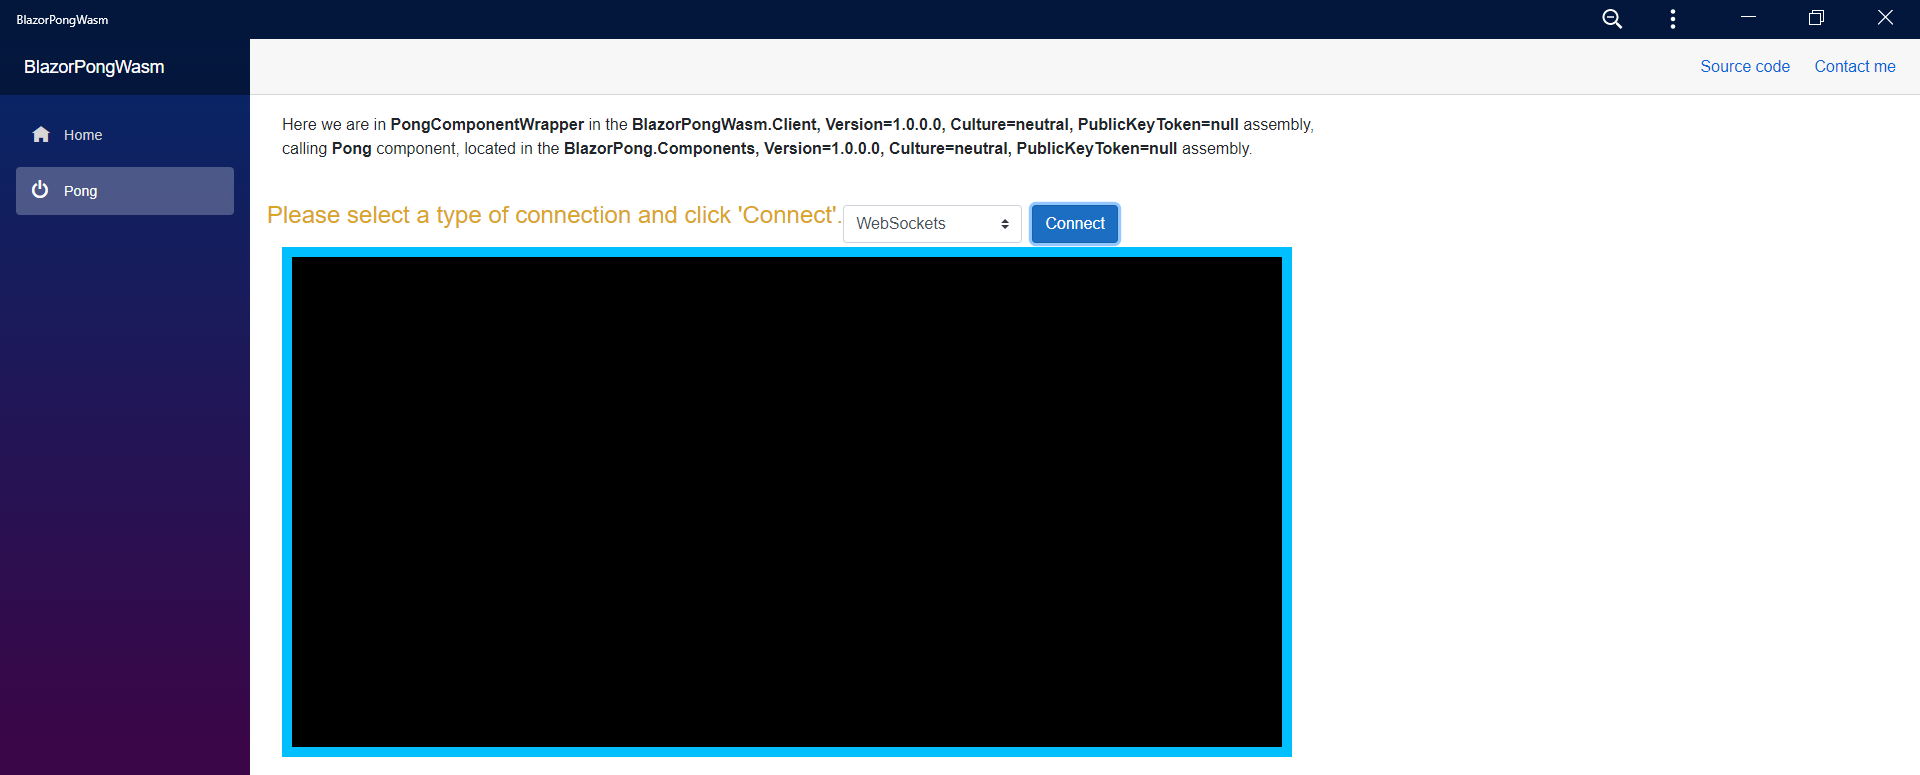
\includegraphics[scale=0.25]{figure/installedBlazorPongWasm.png}}
	\caption{L'applicazione installata ha una sua form dedicata e sembra nativa.}
	\label{fig:installedBlazorPongWasm}
\end{figure}

\pagebreak

\section{Modelli Sperimentali}
\subsection{Blazor Hybrid}\label{sez:bhybrid}
Blazor Hybrid permette di sviluppare applicazioni parzialmente native.
Nel modello Hybrid, l'applicazione sviluppata non \`e quindi pi\`u considerabile un'applicazione web ma rimane ibrida perch\`e pur essendo un'applicazione con capacit\`a native, utilizza tecnologie web per effettuare il rendering della UI.

Esempi di Hybrid Apps possono essere quelle applicazioni mobile native che hanno accesso alle API esposte da Android, ma che utilizzano delle WebViews per la gestione dell'interazione dell'utente con la UI.
Un altro esempio molto interessante sono le applicazioni, scritte in Blazor, che sfruttano Electron.

Electron, precedentemente noto come Atom Shell, \`e un framework open-source sviluppato e mantenuto da GitHub.
In particolare Electron permette di sviluppare interfacce grafiche per desktop eseguibili su Windows, Linux e macOS utilizzando tecnologie web\cite{electronWiki}.
Electron combina il motore di rendering del browser Chromium ed il runtime Node.js, che vengono inclusi in ogni applicazione sviluppata utilizzando questo framework.
Utilizzando quindi il pacchetto NuGet Electron.NET, si pu\`o fare in modo di eseguire un'applicazione .NET Core nell'ambiente(browser e runtime) garantito da Electron, utilizzando Blazor in fase di sviluppo\cite{electronDotNet}.

In questo modo si pu\`o ottenere un'applicazione con capacit\`a native, che sia cross-platform, la cui interfaccia sia stata scritta utilizzando Blazor.
Nella figura \ref{fig:BlazorHybridApplication} si pu\`o vedere una Web Application compilata nativamente con Electron(con target Windows), e quindi eseguita come applicazione desktop:

\begin{figure}[H]
	\centerline{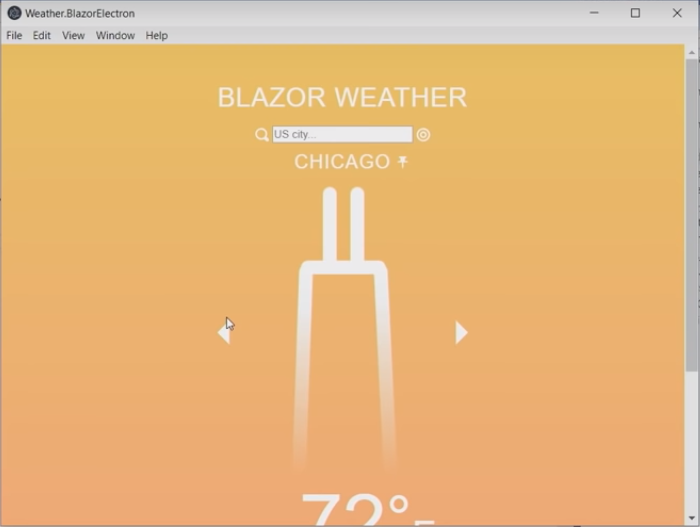
\includegraphics[scale=0.6]{figure/BlazorWeatherElectron.png}}
	\caption{Blazor Hybrid Application}
	\label{fig:BlazorHybridApplication}
\end{figure}

Il codice open source di questa applicazione, si pu\`o trovare al seguente link: https://github.com/danroth27/BlazorWeather/tree/master/BlazorWeather.Electron
\pagebreak

\subsection{Blazor Native}\label{sez:bnative}
Grazie a Blazor Native \`e possibile sviluppare applicazioni completamente native, sfruttando il fatto che Blazor \`e stato architettato per poter renderizzare controlli della UI che non siano obbligatoriamente strumenti web, e pu\`o quindi integrarsi con controlli nativi.
Il rendering layer \`e infatti intercambiabile, pur essendo quello di default dedicato all'HTML.

Un esempio di applicazione sviluppata utilizzando Blazor per il rendering di controlli nativi nella UI, si pu\`o vedere durante la presentazione di Steve Sanderson all'evento NDC ad Oslo del 2019, pur non essendo stato ancora rilasciato il codice di un esempio ufficiale\cite{sandersonNDCBlutter}.
In questa applicazione, si \`e scelto di sostituire il default rendering layer per utilizzarne uno personalizzato, utilizzando componenti di Flutter, il toolkit di Google per costruire interfacce utente native CrossPlatform.
Questo modello viene qui citato per completezza, ma al momento non \`e presente nella documentazione ufficiale ed \`e solo stato citato da Daniel Roth durante la presentazione dei futuri modelli di Blazor sul client\cite{blazorNative}.
Blazor Native \`e quindi da considerare del tutto sperimentale.

\section{Funzionamento}\label{sez:funzionamento}
Quando si scrive codice nei component Blazor, si utilizza un mix di HTML per lo scheletro, CSS per lo stile del documento e C\# preceduto dal relativo carattere di escape(@) per la parte dinamica del codice.
\begin{figure}[H]
	\centerline{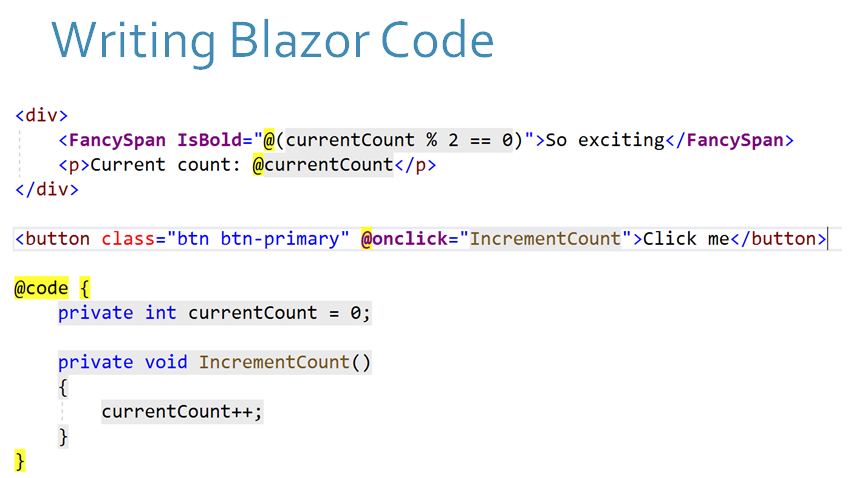
\includegraphics[scale=0.55]{figure/RazorFile.png}}
	\caption{File Razor}
	\label{fig:razorFile}
\end{figure}
Si pu\`o scrivere utilizzando questa sintassi solamente nei file che hanno estensione ".razor", il cui esempio si pu\`o trovare in figura \ref{fig:razorFile}.

Quando l'applicazione viene compilata, i file .razor vengono utilizzati come input per generare dei file C\#(quindi con estensione .cs) equivalenti al codice che si \`e descritto\cite{ryanNowakNDCSydney}.
Un esempio di output di file razor compilato, generato a partire da quello in figura \ref{fig:razorFile} \`e visibile in figura \ref{fig:compiledRazorFile}.
\begin{figure}[H]
	\centerline{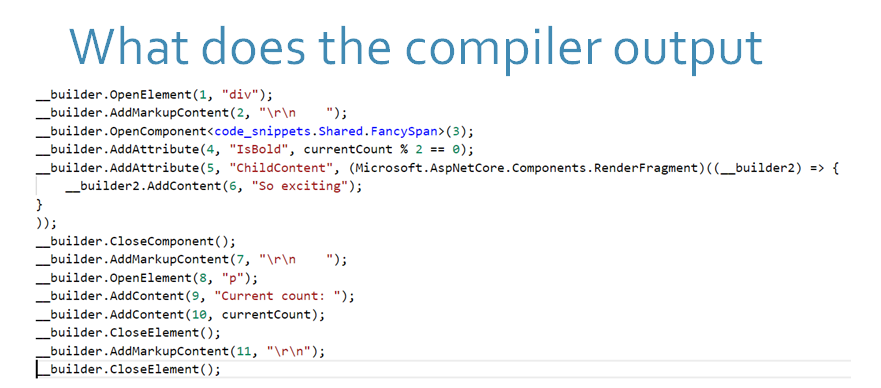
\includegraphics[scale=0.55]{figure/RazorFileCompiled.PNG}}
	\caption{Output}
	\label{fig:compiledRazorFile}
\end{figure}

Saranno poi questi file ad essere effettivamente utilizzati da Roslyn(che \`e il nome del compilatore open-source del linguaggio C\#) e a finire nella DLL generata come output dal progetto nel quale si trova il file .razor di partenza.
Questo passaggio non \`e solo necessario per fare in modo che si possano generare le DLL compilate relative ai file di partenza, ma \`e anche il momento in cui viene ottimizzato ci\`o che ha scritto il developer per ogni parte relativa alla UI in ogni file .razor del progetto, riducendolo alle sole primitive di Blazor, che sono visibili nella figura \ref{fig:BlazorPrimitives}.

\begin{figure}[H]
	\centerline{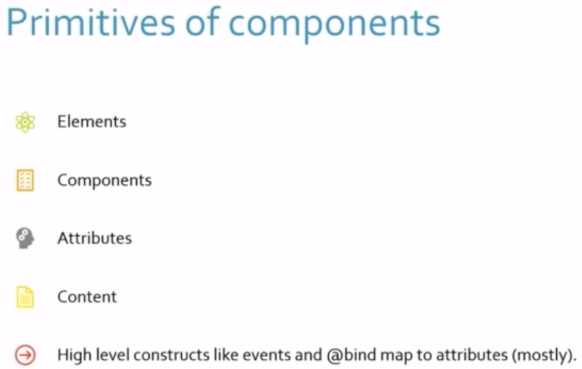
\includegraphics[scale=0.7]{figure/BlazorPrimitives.PNG}}
	\caption{Primitive di Blazor}
	\label{fig:BlazorPrimitives}
\end{figure}

In ordine quindi possiamo descrivere le primitive:
\begin{enumerate}
	\item Un elemento \`e ad esempio l'elemento html "div";
	\item Un component \`e un altro componente(file .razor) che viene utilizzato nel file che si sta compilando;
	\item Un attributo \`e appunto un attributo di un elemento html, o un parametro passato in ingresso ad un component;
	\item Un contenuto \`e del testo, costante o basato su un parametro, inserito all'interno di un elemento html;
	\item L'ultima primitiva di un componente Blazor sono sostanzialmente gli eventi che vengono gestiti dal componente che si sta compilando e le direttive di bind che quindi collegano e mantengono sincronizzate due variabili.
\end{enumerate}

\pagebreak